% Template for Elsevier CRC journal article
% version 1.2 dated 09 May 2011

% This file (c) 2009-2011 Elsevier Ltd.  Modifications may be freely made,
% provided the edited file is saved under a different name

% This file contains modifications for Nuclear Physics B Proceedings Supplement

% Changes since version 1.1
% - added "procedia" option compliant with ecrc.sty version 1.2a
%   (makes the layout approximately the same as the Word CRC template)
% - added example for generating copyright line in abstract

%-----------------------------------------------------------------------------------

%% This template uses the elsarticle.cls document class and the extension package ecrc.sty
%% For full documentation on usage of elsarticle.cls, consult the documentation "elsdoc.pdf"
%% Further resources available at http://www.elsevier.com/latex

%-----------------------------------------------------------------------------------

%%%%%%%%%%%%%%%%%%%%%%%%%%%%%%%%%%%%%%%%%%%%%%%%%%%%%%%%%%%%%%
%%%%%%%%%%%%%%%%%%%%%%%%%%%%%%%%%%%%%%%%%%%%%%%%%%%%%%%%%%%%%%
%%                                                          %%
%% Important note on usage                                  %%
%% -----------------------                                  %%
%% This file should normally be compiled with PDFLaTeX      %%
%% Using standard LaTeX should work but may produce clashes %%
%%                                                          %%
%%%%%%%%%%%%%%%%%%%%%%%%%%%%%%%%%%%%%%%%%%%%%%%%%%%%%%%%%%%%%%
%%%%%%%%%%%%%%%%%%%%%%%%%%%%%%%%%%%%%%%%%%%%%%%%%%%%%%%%%%%%%%

\documentclass[3p,times,procedia]{elsarticle}
\usepackage{nupha_ecrc}


\newcommand{\pp}{pp}
\newcommand{\mpp}{\mathrm{pp}}
\newcommand{\sqrts}{\sqrt{s}}
\newcommand{\sqrtsNN}{\sqrt{s_{\rm NN}}}
\newcommand{\lsim}{\,{\buildrel < \over {_\sim}}\,}
\newcommand{\gsim}{\,{\buildrel > \over {_\sim}}\,}
\newcommand{\av}[1]{\left\langle #1 \right\rangle}
\newcommand{\eV}{\mathrm{eV}}
\newcommand{\keV}{\mathrm{keV}}
\newcommand{\MeV}{\mathrm{MeV}}
\newcommand{\GeV}{\mathrm{GeV}}
\newcommand{\GeVc}{\mathrm{GeV\c}}
\newcommand{\TeV}{\mathrm{TeV}}
\newcommand{\ev}{\mathrm{eV}}
\newcommand{\kev}{\mathrm{keV}}
\newcommand{\mev}{\mathrm{MeV}}
\newcommand{\gev}{\mathrm{GeV}}
\newcommand{\gevc}{\mathrm{GeV}/c}
\newcommand{\tev}{\mathrm{TeV}}
\newcommand{\fm}{\mathrm{fm}}
\newcommand{\mm}{\mathrm{mm}} 
\newcommand{\cm}{\mathrm{cm}}
\newcommand{\m}{\mathrm{m}}
\newcommand{\mum}{\mathrm{\mu m}}
\newcommand{\s}{\mathrm{s}}
\newcommand{\ns}{\mathrm{ns}}
\newcommand{\mrad}{\mathrm{mrad}}
\newcommand{\mb}{\mathrm{mb}}
\newcommand{\mub}{\mathrm{\mu b}}
\newcommand{\T}{\mathrm{T}}
\newcommand{\PbPb}{\mbox{Pb--Pb}}
\newcommand{\pt}{p_{\rm T}}
\newcommand{\dNdy}{{\rm d}N_{ch}/{\rm d}y}
\newcommand{\momwin}{[$p$, $p$+$\Delta$ $p$]}
\newcommand{\DtoKpi}{{\rm D}^0 \to {\rm K}^-\pi^+}
\newcommand{\DtoKpipi}{{\rm D}^+\to {\rm K}^-\pi^+\pi^+}
\newcommand{\DstartoDpi}{{\rm D}^{*+} \to {\rm D}^0 \pi^+}
\newcommand{\DstartoDpiPrecise}{{\rm D^{*+}(2010)\to D^0\pi^+}}
\newcommand{\LctopKzeros}{{\rm \Lambda_{c}^+ \to pK^{0}_{s} \to p\pi^+\pi^-}}
\newcommand{\Dstophip}{{\rm D_{s}^+ \to \phi \pi^+ \to K^{+}K^{-} \pi^+}}
\newcommand{\Dzero}{{\rm D^0}}
\newcommand{\Dzerobar}{\overline{{\rm D^0}}}
\newcommand{\Dstar}{{\rm D^{*+}}}
\newcommand{\Dstarm}{{\rm D^{*-}}}
\newcommand{\Dplus}{{\rm D^+}}
\newcommand{\Dminus}{{\rm D^-}}
\newcommand{\Ds}{{\rm D_{s}^+}}
\newcommand{\Dsminus}{{\rm D_{s}^-}}
\newcommand{\Lc}{{\rm \Lambda_{c}^+}}
\newcommand{\Lcminus}{{\rm \Lambda_{c}^-}}
%\newcommand{\ccbar}{${\rm c}\bar{\rm c}$~}
\newcommand{\nbinv}{{\rm nb^{-1}}}
\newcommand{\decleng}{{\rm L}_{xyz}}
\newcommand{\dEdx}{{\rm d}E/{\rm d}x}
\newcommand{\Pv}{{\rm P}_{\rm v}}
\newcommand{\cubar}{{\rm c}\bar{\rm u}}
\newcommand{\cdbar}{{\rm c}\bar{\rm d}}
\newcommand{\mur}{\mu_{\rm R}}
\newcommand{\muf}{\mu_{\rm F}}
\newcommand{\mc}{m_{\rm c}}
\newcommand{\sigmatot}{\sigma_{\rm tot}}
\newcommand{\ccbar}{${\rm c}\bar{\rm c}$~}
\newcommand{\bbbar}{${\rm b}\bar{\rm b}$~}
\newcommand{\Jpsi}{{\rm J}/\psi}
\newcommand{\RAA}{\rm R_{AA}}

\newcommand{\Ntrk}{N_{\rm tracklets}}
\newcommand{\Nvzero}{N_{\rm VZERO}}
\newcommand{\dNdEta}{{\rm d}N_{\rm ch}/{\rm d}\eta}
\newcommand{\dNdpt}{{\rm d}N^{\rm D}/{\rm d}\pt}
\newcommand{\dNDzdpt}{{\rm d}N^{\rm \Dzero}/{\rm d}\pt}
\newcommand{\dNdydpt}{{\rm d}^2N^{\rm D}/{\rm d}y {\rm d}\pt}
\newcommand{\dNDzdydpt}{{\rm d}^2N^{\rm \Dzero}/{\rm d}y {\rm d}\pt}
\newcommand{\fB}{f_{\rm B}}


\newcommand{\ptjet}{{p}^{\tn{jet ch}}_{\tn{T}}}
\newcommand{\pthf}{{p}_\tn{T}^\tn{HF}}
\newcommand{\etajet}{{\eta}_{\tn{jet}}}
\newcommand{\zch}{{z_{\parallel}^{\tn{ch}}}}
\newcommand{\zchr}{{z_{\parallel\tn{, rec.}}^{\tn{ch}}}}
\newcommand{\zchg}{{z_{\parallel\tn{, gen.}}^{\tn{ch}}}}
\newcommand{\pchjet}{{\bm{p}}^\tn{jet ch}}

\newcommand{\ptjchr}{p_\tn{T, rec.}^\tn{jet ch}}
\newcommand{\ptjchg}{p_\tn{T, gen.}^\tn{jet ch}}
\newcommand{\pth}{p_\tn{T}^\tn{h}}

\newcommand{\tn}[1]{\textnormal{#1}} % normal (upright non-bold) text
\newcommand{\dd}{\mathrm{d}} % total differential symbol

%% The ecrc package defines commands needed for running heads and logos.
%% For running heads, you can set the journal name, the volume, the starting page and the authors

%% set the volume if you know. Otherwise `00'
\volume{00}

%% set the starting page if not 1
\firstpage{1}

%% Give the name of the journal
\journalname{Nuclear Physics A}

%% Give the author list to appear in the running head
%% Example \runauth{C.V. Radhakrishnan et al.}
\runauth{}

%% The choice of journal logo is determined by the \jid and \jnltitlelogo commands.
%% A user-supplied logo with the name <\jid>logo.pdf will be inserted if present.
%% e.g. if \jid{yspmi} the system will look for a file yspmilogo.pdf
%% Otherwise the content of \jnltitlelogo will be set between horizontal lines as a default logo

%% Give the abbreviation of the Journal.
\jid{nupha}

%% Give a short journal name for the dummy logo (if needed)
\jnltitlelogo{Nuclear Physics A}

%% Hereafter the template follows `elsarticle'.
%% For more details see the existing template files elsarticle-template-harv.tex and elsarticle-template-num.tex.

%% Elsevier CRC generally uses a numbered reference style
%% For this, the conventions of elsarticle-template-num.tex should be followed (included below)
%% If using BibTeX, use the style file elsarticle-num.bst

%% End of ecrc-specific commands
%%%%%%%%%%%%%%%%%%%%%%%%%%%%%%%%%%%%%%%%%%%%%%%%%%%%%%%%%%%%%%%%%%%%%%%%%%

%% The amssymb package provides various useful mathematical symbols
\usepackage{amssymb}
%% The amsthm package provides extended theorem environments
%% \usepackage{amsthm}

%% The lineno packages adds line numbers. Start line numbering with
%% \begin{linenumbers}, end it with \end{linenumbers}. Or switch it on
%% for the whole article with \linenumbers after \end{frontmatter}.
%% \usepackage{lineno}

%% natbib.sty is loaded by default. However, natbib options can be
%% provided with \biboptions{...} command. Following options are
%% valid:

%%   round  -  round parentheses are used (default)
%%   square -  square brackets are used   [option]
%%   curly  -  curly braces are used      {option}
%%   angle  -  angle brackets are used    <option>
%%   semicolon  -  multiple citations separated by semi-colon
%%   colon  - same as semicolon, an earlier confusion
%%   comma  -  separated by comma
%%   numbers-  selects numerical citations
%%   super  -  numerical citations as superscripts
%%   sort   -  sorts multiple citations according to order in ref. list
%%   sort&compress   -  like sort, but also compresses numerical citations
%%   compress - compresses without sorting
%%
%% \biboptions{comma,round}

% \biboptions{}

% if you have landscape tables
\usepackage[figuresright]{rotating}

% put your own definitions here:
%   \newcommand{\cZ}{\cal{Z}}
%   \newtheorem{def}{Definition}[section]
%   ...

% add words to TeX's hyphenation exception list
%\hyphenation{author another created financial paper re-commend-ed Post-Script}

% declarations for front matter

\begin{document}

\begin{frontmatter}

%% Title, authors and addresses

%% use the tnoteref command within \title for footnotes;
%% use the tnotetext command for the associated footnote;
%% use the fnref command within \author or \address for footnotes;
%% use the fntext command for the associated footnote;
%% use the corref command within \author for corresponding author footnotes;
%% use the cortext command for the associated footnote;
%% use the ead command for the email address,
%% and the form \ead[url] for the home page:
%%
%% \title{Title\tnoteref{label1}}
%% \tnotetext[label1]{}
%% \author{Name\corref{cor1}\fnref{label2}}
%% \ead{email address}
%% \ead[url]{home page}
%% \fntext[label2]{}
%% \cortext[cor1]{}
%% \address{Address\fnref{label3}}
%% \fntext[label3]{}

%% Instructions from Editor: Please use the following \dochead only in the preprint version (e-print arXiv etc.); 
%% use empty \dochead{} when submitting to Nuclear Physics A!
\dochead{XXVIIIth International Conference on Ultrarelativistic Nucleus-Nucleus Collisions\\ (Quark Matter 2019)}
%\dochead{}
%% Use \dochead if there is an article header, e.g. \dochead{Short communication}
%% \dochead can also be used to include a conference title, if directed by the editors
%% e.g. \dochead{17th International Conference on Dynamical Processes in Excited States of Solids}

\title{Latest results on $\Lc$ and D production in pp and Pb-Pb collisions at $\sqrtsNN$ = 5.02 TeV with ALICE at the LHC}

%% use optional labels to link authors explicitly to addresses:
%% \author[label1,label2]{<author name>}
%% \address[label1]{<address>}
%% \address[label2]{<address>}

\author{Gian Michele Innocenti}

\address{CERN, Espl. des Particules 1, 1211 Meyrin, Switzerland}

\begin{abstract}
The measurement of heavy-flavour production represents a powerful tool to study the medium formed in high-energy 
heavy-ion collisions. Produced in hard scattering processes on a timescale shorter than the QGP formation time, 
they experience the whole evolution of the medium interacting with its constituents. The measurements of charm-hadron 
production allows testing the mechanisms of in-medium parton energy loss. Moreover, the study of charm-baryon 
production in heavy-ion collisions and in particular the baryon-to-meson ratio, provides unique information on 
hadronisation mechanisms, constraining the role of coalescence.
In this contribution, the ALICE results on open charmed meson and baryon production in large and small systems will be presented
with a focus on the recent measurements of $\Lc$/$\Dzero$ and $\Ds$/$\Dzero$ ratios in central and peripheral PbPb collisions 
and on the new results obtained for the same ratios in proton-proton collisions as a function of the charged particle multiplicity.
The prospects for $\Xi_{c}$ and $\Sigma_{c}$ analyses will also be discussed.
\end{abstract}

\begin{keyword}
Heavy ions \sep heavy flavours \sep energy loss \sep quark recombination
\end{keyword}
\end{frontmatter}

%%
%% Start line numbering here if you want
%%
% \linenumbers

%% main text
\section{Introduction}
\label{intro}
Charm and beauty quarks are produced in hard scattering processes at the very early stages of heavy-ion collisions. As a consequence of the 
large momentum transferred in these processes, their production can be effectively described by perturbative QCD calculations. 
Once produced, these probes traverse the hot and dense medium and interact with the medium constituents via inelastic and elastic processes.
Therefore, by studying their suppression in heavy-ion collisions relative to the vacuum, one can investigate the microscopic nature of energy loss processes
and constrain fundamental parameters of the system, such as the charm diffusion coefficient. Alternatively, measurements of 
heavy-flavour hadrochemistry can be used to constrain the relevance of of quark recombination processes in the medium.
The study of heavy-flavour production can also play an important role in understanding the nature of the systems created in proton-proton and 
proton-lead collisions. Measurements of heavy-particle ratios can highlight the presence of recombination 
processes in small systems and shed new light into the medium-like phenomena that have been observed over the last years, both at RHIC and at the LHC. 
A more detailed description of heavy-flavour physics in large and small systems can be found in~\cite{saporegravis,prinorapp,yenjie}.

\section{Heavy-quark energy loss}
\label{eloss}
With the large statistics collected at the end of 2018, ALICE was able to update its measurements of the nuclear modification factors of 
non-strange D mesons in central and peripheral Pb--Pb collisions. In Fig.~\ref{fig:prompt_nonpromptRAA} (left), the $\RAA$ of non-strange D mesons in the centrality 
interval of 0--10$\%$ is presented as a function of the transverse momentum, $\pt$. For the first time at the LHC, the $\Dzero$ production is measured 
in central collisions down to 0 GeV/$\it{c}$. Thanks to its high accurcay, this measurement is now capable of challenging energy-loss calculations in a wide 
transverse momentum region~\cite{bamps,tamu,phsd,sHQ,catania}. In addition, the new data point obtained in the 0--1 $\GeV$/$\it{c}$ bin provides new experimental constraints on the relevance of 
shadowing in the charm sector. A new measurement of beauty suppression via the analysis of non-prompt $\Dzero$ hadrons 
was also presented. In the middle panel of Fig.~\ref{fig:prompt_nonpromptRAA}, the ratio of the $\RAA$ of non-prompt and prompt $\Dzero$ mesons is shown
as a function of $\pt$. The ratio shows a maximum for $\pt \sim$10 $\GeV$/$\it{c}$ and decreases at higher transverse momenta. This trend is well 
described by theoretical calculations which include a different energy loss for charm and beauty quarks~\cite{tamu,sHQ,cujet3}. 

\section{Charm recombination}
\label{recombination}
Stronger constraints on the role of charm recombination were obtained thanks to new measurements of the $\Ds$/$\Dzero$ and $\Lc$/$\Dzero$ ratios
in central Pb--Pb collisions. In Fig.~\ref{fig:prompt_nonpromptRAA} (right), the double ratio of $\Ds$/$\Dzero$ measured in Pb--Pb and pp collisions 
is presented as a function of $\pt$. An enhancement of a factor of approximately 2 is observed in central Pb--Pb collisions at $\pt$ of $\approx$5 $\GeVc$/$\it{c}$. The $\pt$-dependence and magnitude 
of this enhancement are well described by theoretical calculations, like TAMU, that adopt a Langevin approach to describe the charm evolution in the 
medium whilst also including charm recombination~\cite{tamu}. The first measurement of the $\Lc$/$\Dzero$ ratio in central Pb--Pb collisions was also presented. 
In the left panel of Fig.~\ref{fig:LcD0andtheory}, the Pb--Pb measurement performed in the centrality region of 0--10$\%$ is presented and compared to the same ratio
measured in semi-peripheral Pb--Pb and pp collisions. A moderate enhancement is observed in central and peripheral collisions with respect to pp for $\pt$ of about 5--8 $\GeVc$/$\it{c}$,
as expected in the presence of charm recombination. In the right panel of the same plot, the central Pb--Pb measurement is compared to different theoretical calcuations~\cite{catania,shm,pythia8}.
More precise measurements will be needed in order to be able to discriminate amongst different theoretical descriptions of this observable.
\begin{figure}[h]
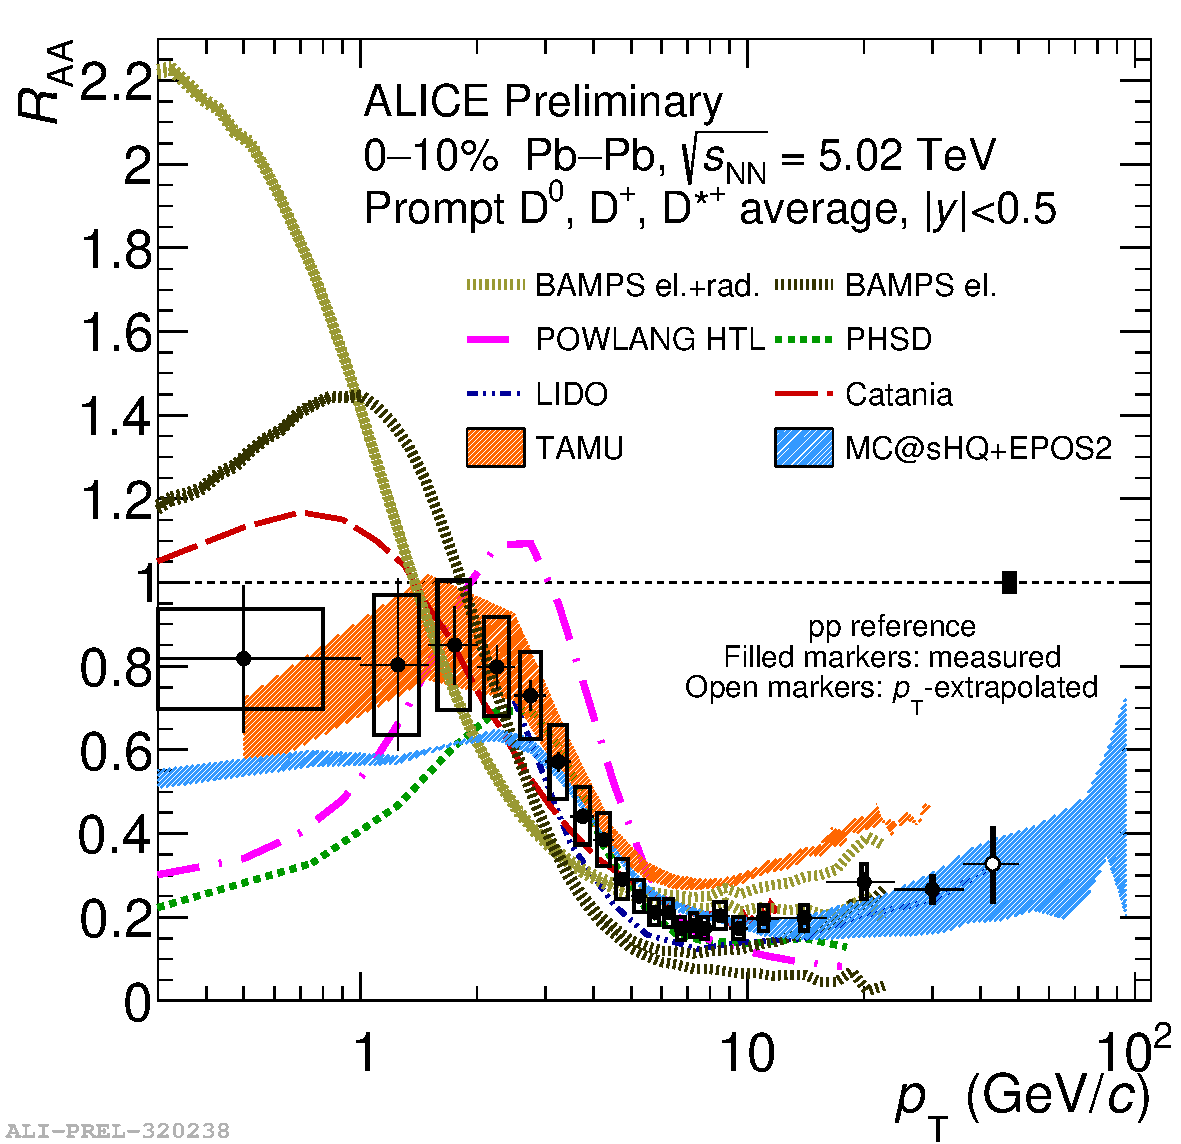
\includegraphics[width=0.33\textwidth]{Plots/D/2019-10-31-2019-10-28-DmesonAverage_vs_transportmodels_010_5dot02.pdf}
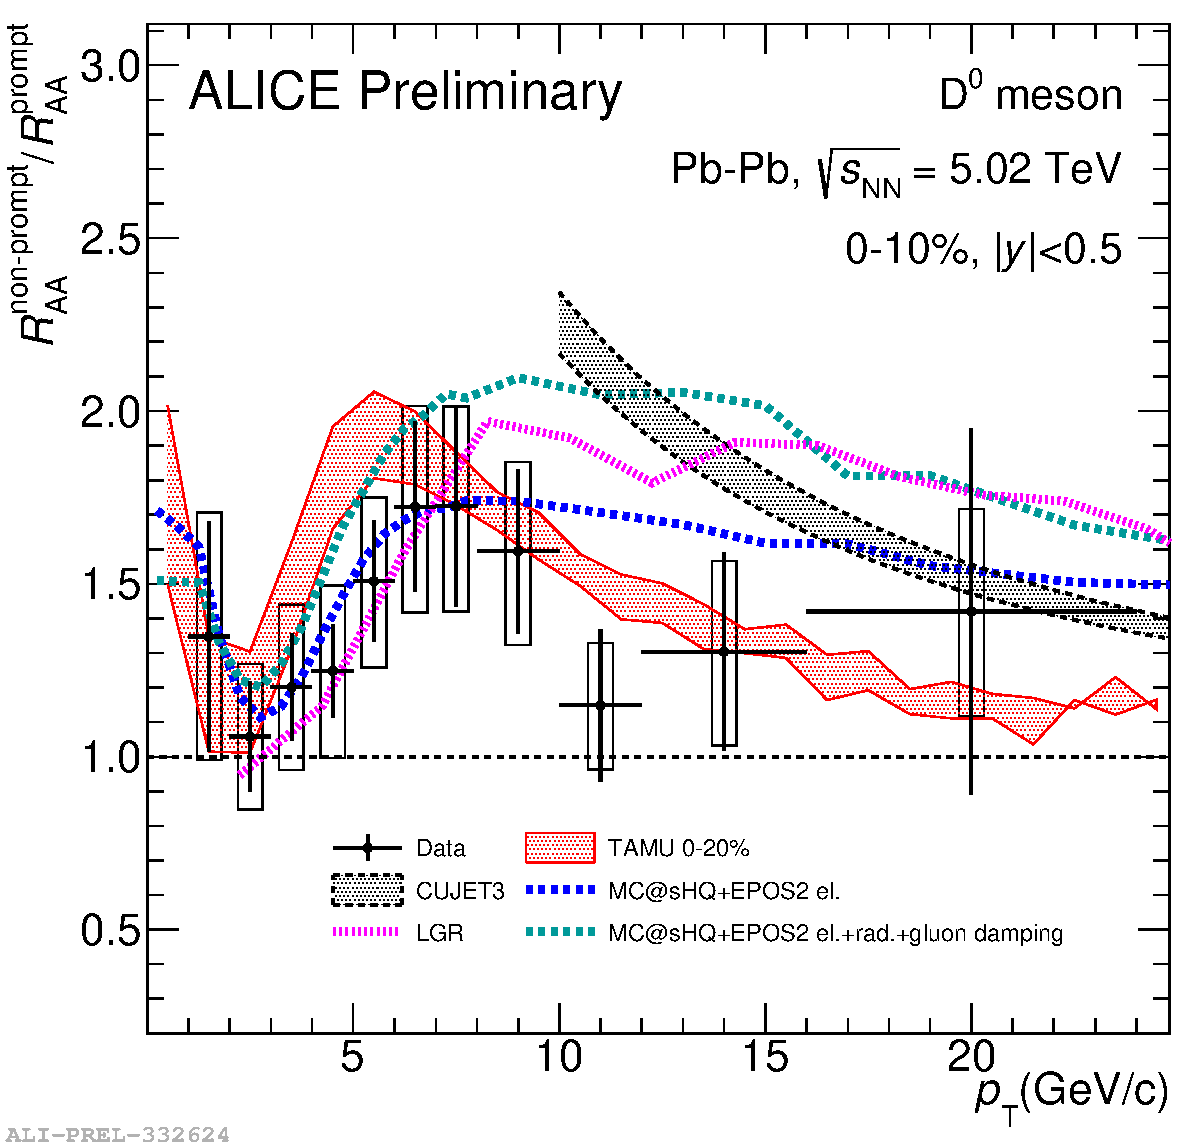
\includegraphics[width=0.33\textwidth]{Plots/NP/2019-10-31-2019-10-29-D0PbPb5TeV_010_RaaRatio_wModel.pdf}
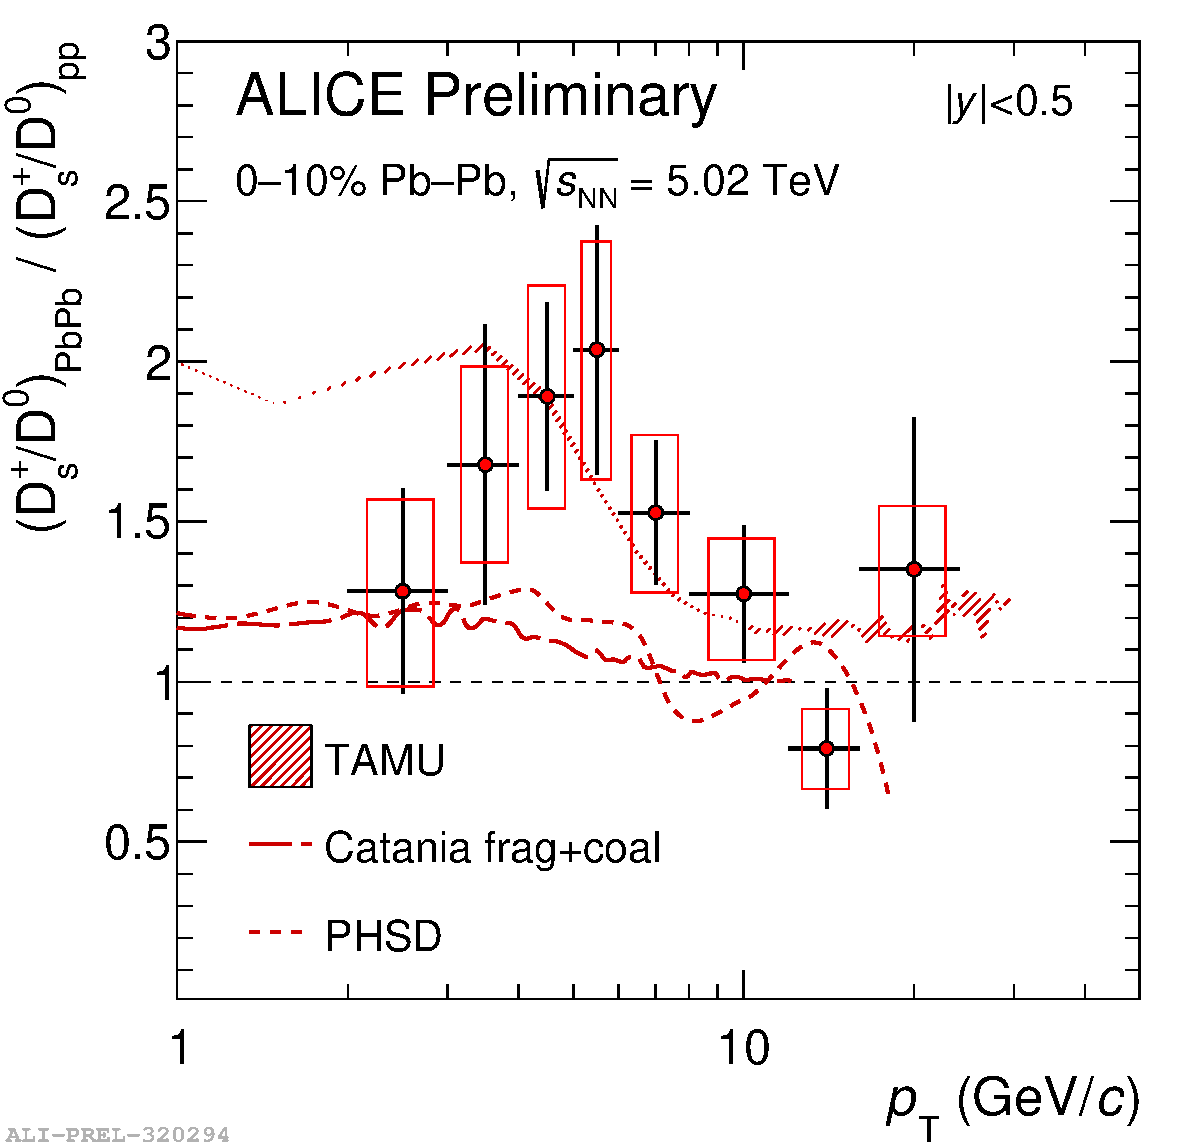
\includegraphics[width=0.33\textwidth]{Plots/D/2019-10-31-2019-10-28-DoubleRatio_DsOverDzero_PbPb2018_010_pp_WithModels.pdf}
\caption{(Left) $\RAA$ of non-strange D mesons in the centrality interval of 0--10$\%$ is compared to various theoretical calculations. 
	(Middle) Ratio of the $\RAA$ of non-prompt and prompt $\Dzero$ mesons as a function of $\pt$. 
	(Right) Double ratio of $\Ds$/$\Dzero$ measured in central Pb--Pb and pp collisions.}
\label{fig:prompt_nonpromptRAA}
\end{figure}

\section{Heavy-flavour hadronization in small systems}
\label{recombination}
The comparison between the $\Ds$/$\Dzero$ and $\Lc$/$\Dzero$ ratios in pp and central Pb--Pb collisions, despite the limited statistical precision, 
supports the hypothesis of baryon/meson ehancement due to charm recombination inside the QGP. The natural extension was to therefore
understand whether these phenomena could also play a role in small systems.
In this conference, the first measurements of the $\Ds$/$\Dzero$ and $\Lc$/$\Dzero$ ratios as a function of multiplicity in pp collisions were presented.
For these measurements, the multiplicity was sampled according to the number of tracklets measured in the two innermost layers of the Inner Tracking 
System (ITS). The lowest multiplicity range considered corresponds to an average $\rm dN_{ch}/d\eta$ of 3.9, well below the average pp multiplicity, whilst 
the highest interval has an average $\rm dN_{ch}/d\eta$ of about 2.5 times that of the minimum-bias one.
In the left panel of Fig.~\ref{fig:highmult}, the $\Ds$/$\Dzero$ ratios as a function of $\pt$ in different ranges of charged particle multiplicity are presented. 
For this ratio, a mild increase still not statistically significant is observed at intermediate $\pt$. 
However, as shown in the right panel of the same figure, a much stronger multiplicity dependence is observed 
for the $\Lc$/$\Dzero$ ratio. At a theoretical level no framework for recombination in pp is available. However, the comparison with PYTHIA calculations provides some very interesting information. Even at the lowest multiplicities, the ratio in data is already enhanced compared to the standard PYTHIA Monash tune which describes the $^+$e$^-$ measurements. To capture the multiplicity dependence seen in data the PYTHIA tune is varied to include more processes of colour reconnection beyond leading colour~\cite{pythia8CR}. In this formalism, the enhancement compared to the $^+$e$^-$ baseline could be attributed to
final state colour reconnection processes that do not strictly require the presence of a QGP. 
New and higher precision measurements along with further comparisons to theoretical calculations are still needed in order to draw a firm conclusion. One such measurement is the ratio of $\Xi^{0}_{c}/\Dzero$ in pp collisions, which was also presented (Fig.~\ref{fig:future}). Here the measured ratio is largely underestimated by PYTHIA even when colour recombination effects are enhanced, suggesting that such a variable could have a stronger discrimination power to study
these phenomena.  
\begin{figure}[h]
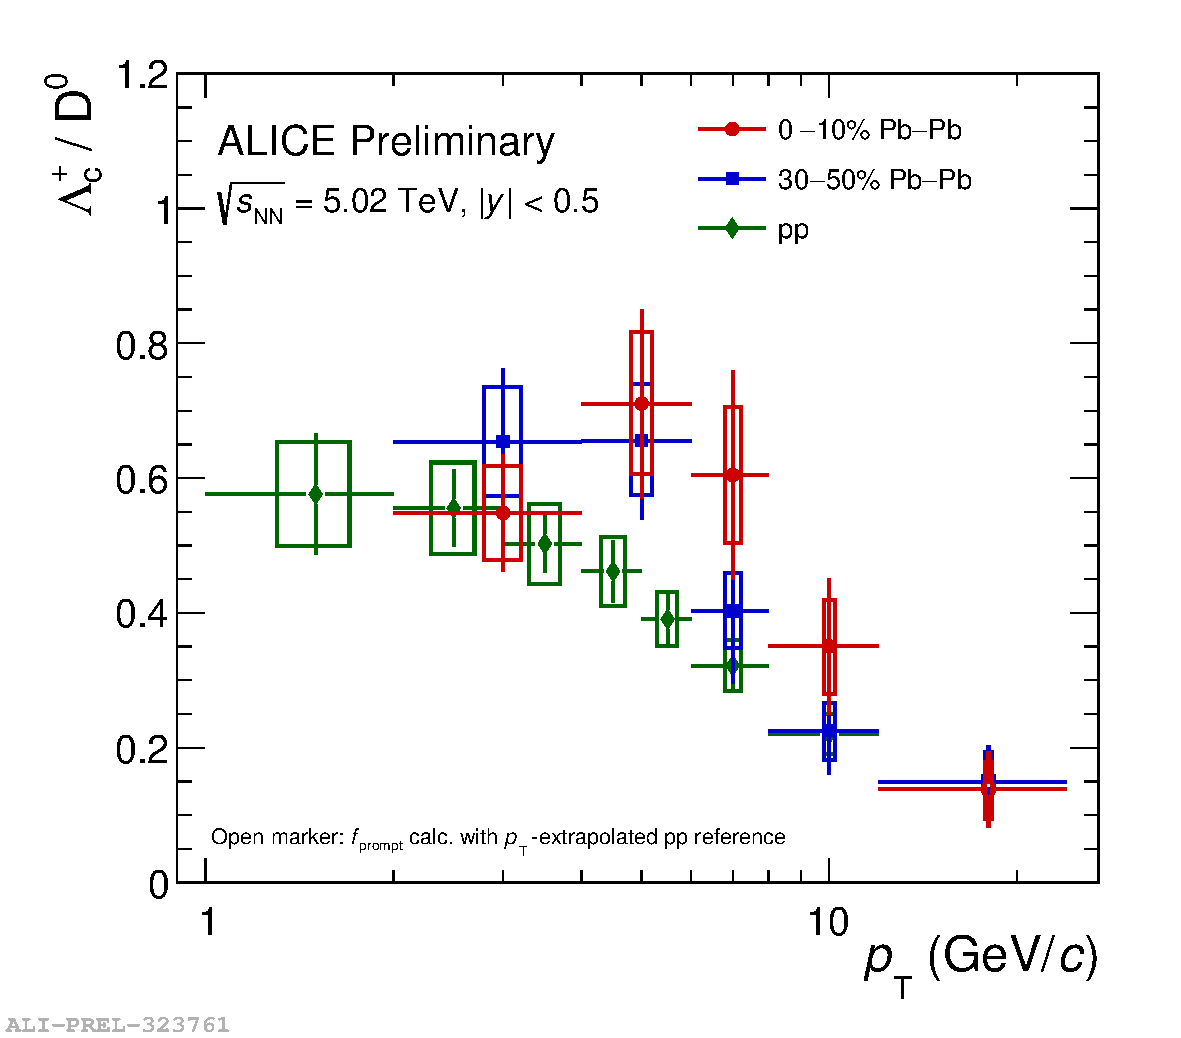
\includegraphics[width=0.43\textwidth]{Plots/PbPbLc/2019-10-28-LcD_PbPb18_010_3050_pp_Logx_shift.pdf}
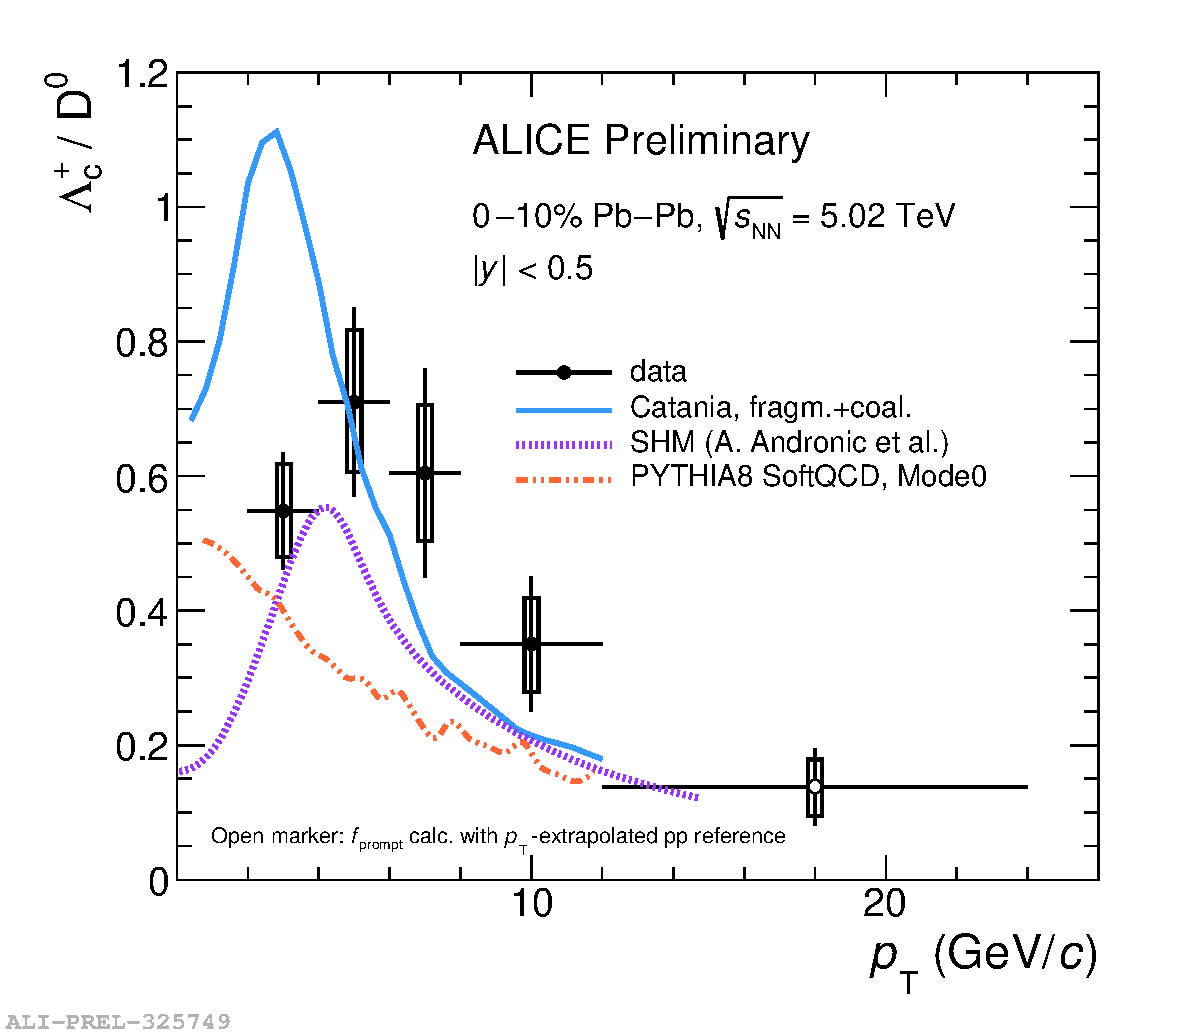
\includegraphics[width=0.43\textwidth]{Plots/PbPbLc/2019-10-31-LcD_PbPb18_010_theory_withPythia.pdf}
\caption{
	(Left) Ratio of the $\RAA$ of $\Lc$ and $\Dzero$ mesons as a function of $\pt$ in pp, central and semipheripheral PbPb collisions. 
	(Right) Ratio of the $\RAA$ of $\Lc$ and $\Dzero$ mesons in central PbPb collisions compared to theoretical calculations.}
\label{fig:LcD0andtheory}
\end{figure}

\begin{figure}[h]
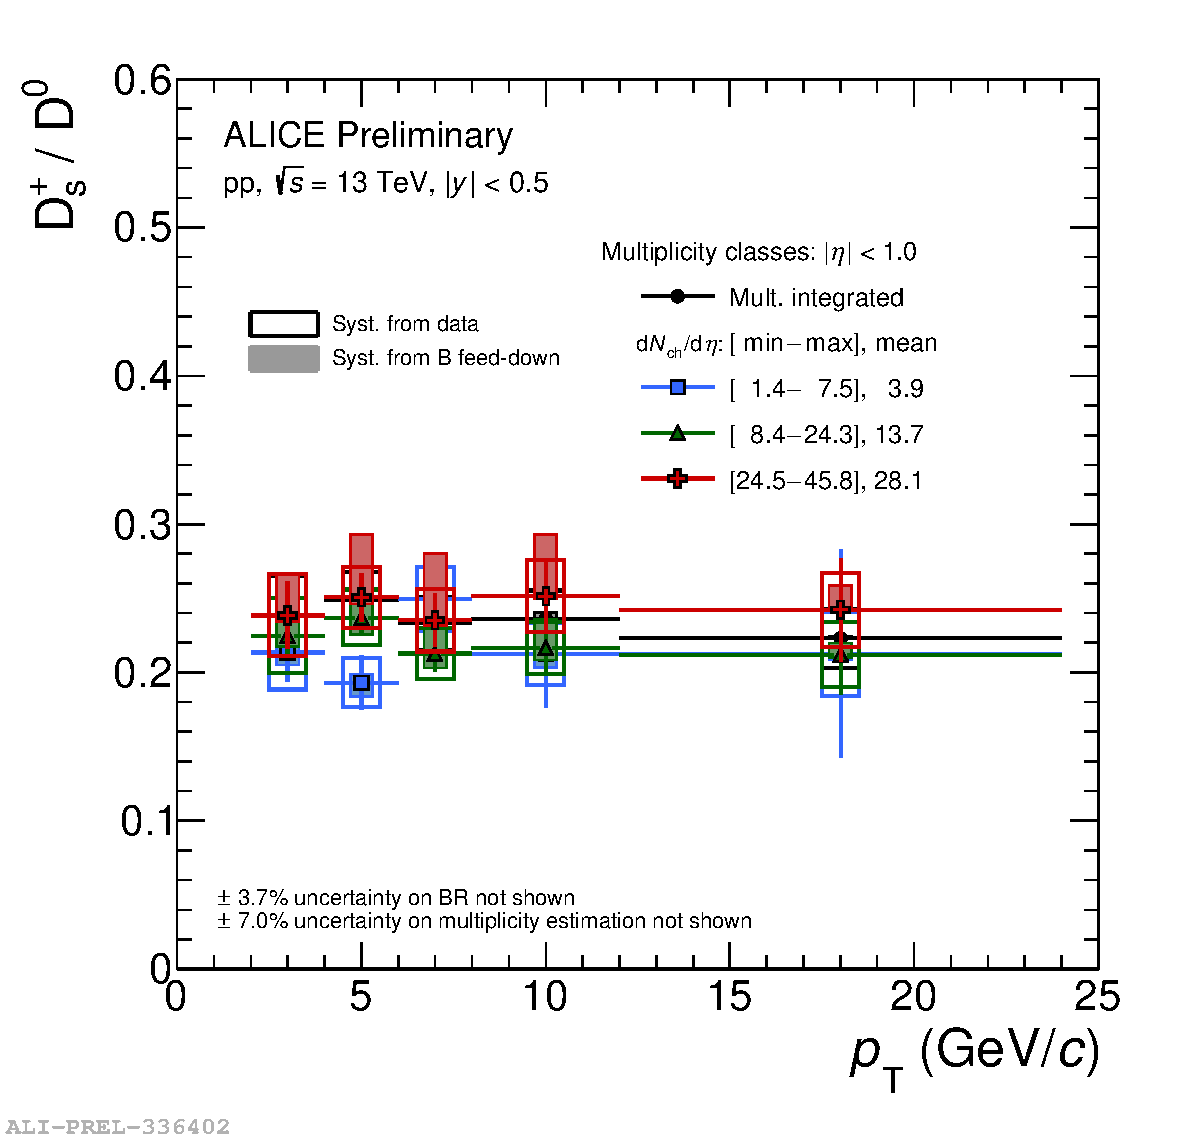
\includegraphics[width=0.43\textwidth]{Plots/ppHM/2019-10-31-2019-10-31-DsOverD0_allMult_MB.pdf}
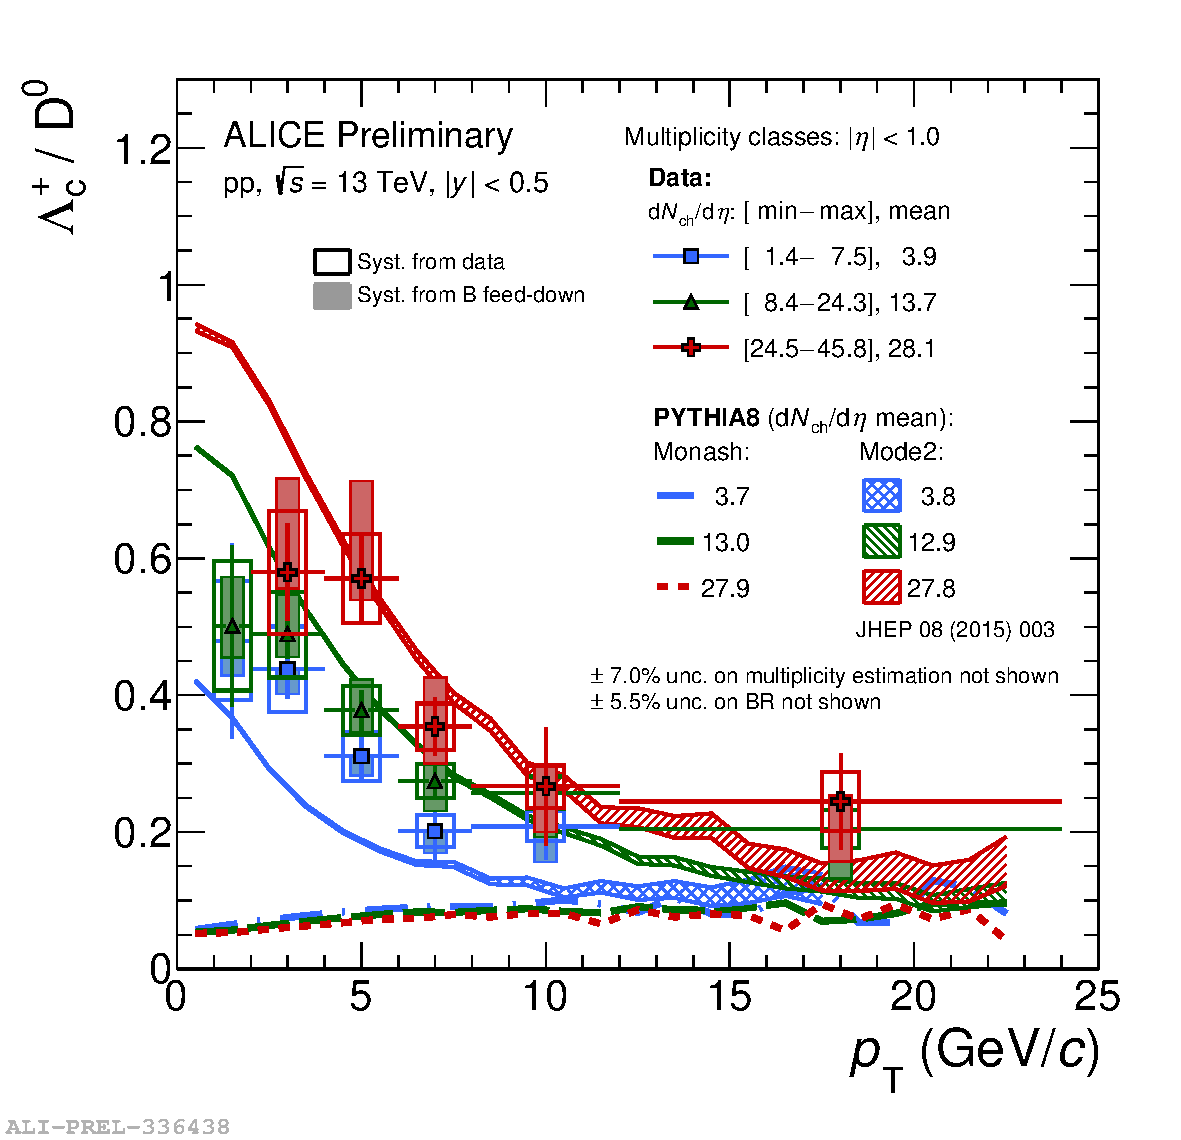
\includegraphics[width=0.43\textwidth]{Plots/ppHM/2019-10-31-2019-10-31-LcpKpiOverD0_wPythiaMonashMode2_allMult.pdf}
\caption{
	(Left) $\Ds$/$\Dzero$ ratio measured in pp collisions at 13 TeV in different multiplicity intervals. 
	(Right) $\Lc$/$\Dzero$ ratio measured in pp collisions at 13 TeV in different multiplicity intervals compared to different PYTHIA calculations.} 
\label{fig:highmult}
\end{figure}
\begin{figure}[h]
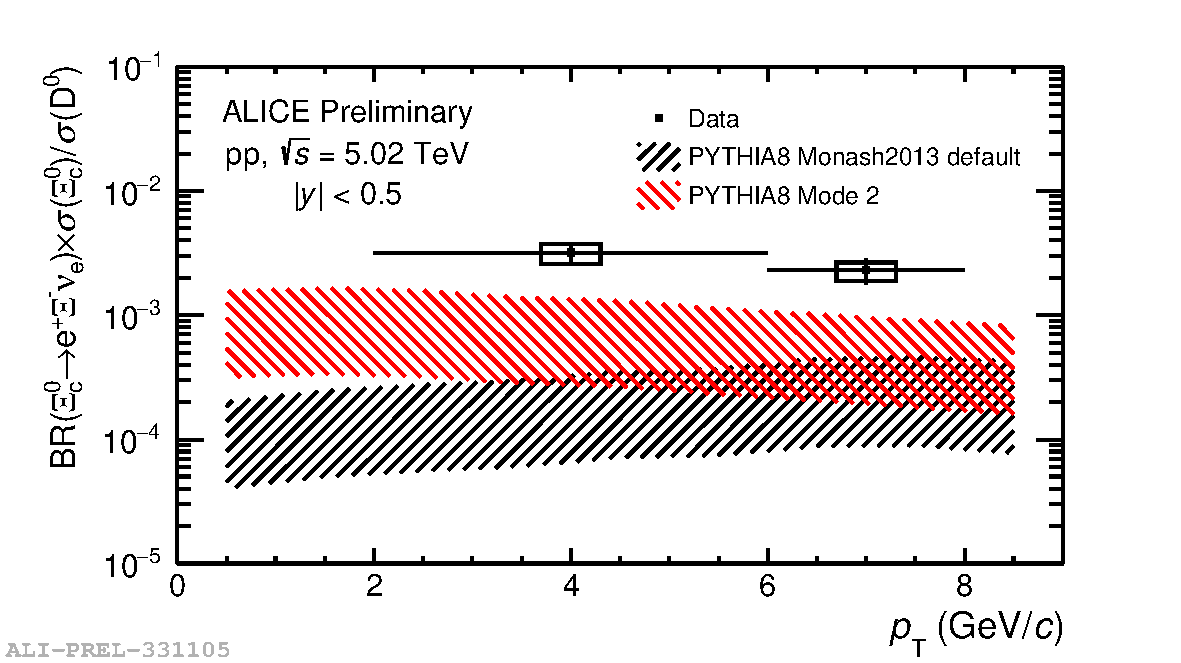
\includegraphics[width=0.76\textwidth]{Plots/Xi_c/2019-10-28-2019-10-28-Xic0toD0_5TeV_wModel1.pdf}
\caption{$\Xi_{c}$/$\Dzero$ ratio measured in pp collisions at 5 TeV compared to PYTHIA calculations.}
\label{fig:future}
\end{figure}

%% The Appendices part is started with the command \appendix;
%% appendix sections are then done as normal sections
%% \appendix

%% \section{}
%% \label{}

%% References
%%
%% Following citation commands can be used in the body text:
%% Usage of \cite is as follows:
%%   \cite{key}         ==>>  [#]
%%   \cite[chap. 2]{key} ==>> [#, chap. 2]
%%

%% References with BibTeX database:

\bibliographystyle{elsarticle-num}
\bibliography{<your-bib-database>}

%% Authors are advised to use a BibTeX database file for their reference list.
%% The provided style file elsarticle-num.bst formats references in the required Procedia style

%% For references without a BibTeX database:

 \begin{thebibliography}{00}

%%   \bibitem{key}...
%%

% \bibitem{}
\bibitem{saporegravis} A. Andronic et al., Eur. Phys. J. C 76 (2016) 107, doi:10.1140/epjc/s10052-015-3819-5, arXiv:1506.03981.
\bibitem{prinorapp} F. Prino, R. Rapp, Journal of Physics G: Nuclear and Particle Physics, Vol.3, Num. 9, 10.1088/0954-3899/43/9/093002, arXiv:1603.00529.
\bibitem{yenjie} X. Dong, Y-J. Lee, R. Rapp, Annual Review of Nuclear and Particle Science, Vol. 69:417-445, arXiv:1903.07709.
\bibitem{bamps} Uphoff J, Fochler O, Xu Z, Greiner C. J. Phys. G42:115106 (2015).
\bibitem{tamu} He M, Fries RJ, Rapp R. Phys. Lett. B735:445 (2014).
\bibitem{phsd} Song T, et al. Phys. Rev. C93:034906 (2016).
\bibitem{sHQ} Andronic A, et al. Eur. Phys. J. C76:107 (2016).
\bibitem{catania} Das SK, Scardina F, Plumari S, Greco V. Phys. Lett. B747:260 (2015).
\bibitem{cujet3} A. Buzzatti, M. Gyulassy, arXiv:1207.6020.
\bibitem{shm} A.Andronic,P.Braun-Munzinger,K.RedlichandJ.Stachel,Nucl.Phys.A789(2007)334,arXiv:nucl-th/0611023.
\bibitem{pythia8} An introduction to PYTHIA 8.2, https://doi.org/10.1016/j.cpc.2015.01.024.
\bibitem{pythia8CR} J. R. Christiansen, P. Z. Skands, arXiv:1505.01681.
\end{thebibliography}

\end{document}

%%
%% End of file `nupha-template.tex'.
